% !TEX root = ../main.tex

\chapter{Deep learning}
\label{ch:deep_learning}

\section{Introduction to deep learning}
Deep learning is currently one of the trendiest topics in machine learning, a subset of artificial intelligence. Machine learning refers to statistical models that allow computers to perform specific tasks without having been explicitly programmed to solve them. In fact, these models try to find structural patterns within data in order to understand new incoming situations and react in the best possible way accordingly. There exist various techniques in machine learning such as k-NN, SVM, k-means, decision trees, association rules, etc. What mainly differentiates deep learning from these algorithms is the concept of neural networks (see section  \ref{what_is_a_neural_network}), that are combined to form deep neural networks.\\
Neural networks are inspired from the biological neural networks of the brain. These systems try to learn how to solve a problem based on the data they receive as input. Many concrete applications make use of neural networks: autonomous vehicles, smarter translators, computer-aided diagnoses, personal assistants, art creation, robotics, etc. The presence of deep learning techniques in all mentioned use cases clearly attests that this technology is a real breakthrough. Furthermore, since this field has recently gained interest   (see section \ref{historical_background}), multiple researches are still ongoing, which suggests that many exciting new applications will certainly be discovered.

\subsection{Historical background}
\label{historical_background}
As described in figure \ref{history} from article \cite{14}, the theoretical foundations of deep learning appeared long before the invention of the computers. From the first attempts to understand the human brain until today, a long way has been made to establish the basic components of modern neural networks. One could ask: why did deep learning take off recently if the theory has been around for a long time?\\
First part of the answer is about the computational power. Indeed, deep learning algorithms need a lot of data to work properly and this requires powerful CPU/GPU that either didn't exist or were only available to a minority of people. One other main reason concerns the lack of data. Since deep learning algorithms "learn" from data, if not data is available, no learning is possible. Consequently, the era of Big Data has enhanced the deep learning possibilities. These two points are summarised: "The increase in model size overtime, due to the availability of faster CPUs, the advent of general purpose GPUs, fasternetwork, connectivity and better software infrastructure for distributed computing, is one of the most important trends in the history of deep learning. This trend is generally expected to continue well into the future"\cite{15}.\\
Finally, before the year 2012, the abilities of neural networks had not been publicly proven. This changed with the ImageNet Large Scale Visual Recognition Challenge (a competition where researchers evaluate their algorithms on several visual recognition tasks). In fact, the deep convolutional neural network called "AlexNet" achieved 16\% of classification error rate, whereas the previous best scores were around 25\%. This victory marked the beginning of a new craze for these types of algorithms.



\begin{figure}[!h]
\centering
\includegraphics[width=1\textwidth, keepaspectratio=true]{./figures/history.png}
\caption{Milestones }
\label{history}
\end{figure}

 
\subsection{What is a neural network?}
\label{what_is_a_neural_network}

From a descriptive point of view, neural networks can simply be seen as a non linear applications that associate an input to an output with respect to certain parameters. The input can be images, sounds or whatever features that is numerical. The output of a neural network depends on the problem it tries to solve. In computer vision, the most common types of outputs  are classes (for classification problems) and pixel coordinates (for segmentation problems).\\
From a mathematical point of view, a neural network can be defined as a non linear function $f$ that associates to an input $x$ an output $y$ with respect to parameters $\theta$.
\begin{equation}
y = f(x,\theta)
\end{equation}
The parameters $\theta$ are estimated from the training samples.
%\begin{figure}[!h]
%\centering
%\includegraphics[width=1\textwidth, keepaspectratio=true]{./figures/neural_network.png}
%\caption{Neural Network example}
%\label{neural_network}
%\end{figure}





\section{Neural networks basics}

\subsection{Notation}
In order to respect a consistent mathematical notation to describe neural networks, this work will use the notation of Andrew Y. Ng, one of the pioneers of deep learning, that can be found in \cite{16}.\\

\noindent \textbf{General comment}
\begin{itemize}
\item Superscript (i) will denote the $i^{th}$ training example.
\item Superscript [l] will denote the $l^{th}$ layer of the neural network.
\end{itemize}

\noindent \textbf{Sizes}
\begin{itemize}
\item $m$: number of examples in the dataset.
\item $n_{x}$: input size.
\item $n_{y}$: output size (or number of classes).
\item $n_{h}^{[l]}$: number of hidden units (i.e neurons) of the $l^{th}$ layer. 
\item $L$: number of layers in the network.
\end{itemize}

\noindent \textbf{Neural networks components}
\begin{itemize}
\item $X\in \R$ is the input matrix matrix of a neural network.
\item $x^{(i)} \in \R^{n_{x}}$ is the $i^{th}$ example (sample) represented as a column vector.
\item $Y \in \R^{n_{y} \times m}$ is the label matrix.
\item $y^{(i) \in \R^{n_{y}}}$ is the output label for the $i^{th}$ example.
\item $W^{[l]} \in \R$ \textsuperscript{\# of neurons in the next layer = j  x \# of neurons in the previous layer = k} is the weight matrix at layer $[l]$.
\item $b^{[l]} \in R$\textsuperscript{\# of units in next layer} is the bias vector in the $l^{th}$ layer.
\item $\hat{y} \in R^{n_{y}}$ is the predicted output vector. It can also be denoted $a^{[L]}$ where $L$ is the number of layers in the network.
\item $g^{[l]}(x)$ is the $l^{th}$ activation function.  
\item $z^{[l]} = W_{x}x^{(i)} + b^{[l]}$ denotes the weighted sum of the input given to the $l^{th}$ layer before passing through the activation function.\\
\end{itemize}

\noindent \textbf{Forward propagation equations}
\begin{itemize}
\item $a = g^{[l]}(W_{x}x^{(i)} + b^{[l]}) = g^{[l]}(z^{[l]})$ where $g^{[l]}$ denotes the $l^{th}$ layer activation function.
\item $a_{j}^{[l]} = g^{[l]} (\sum_{k} w_{jk}^{[l]}a_{k}^{[l-1]} + b_{j}^{[l]}) = g^{[l]} (z_{j}^{[l]}) $ is the general activation formula at $l^{th}$ layer.
\item $J(x, W, b, y) or J(\hat{y}, y)$ denote the cost function.
\end{itemize}

\subsection{Perceptrons}
\label{perceptron}
Perceptrons are the main components of neural networks. They were "developed in the 1950s and 1960s by the scientist Frank Rosenblatt, inspired by earlier work by Warren McCulloch and Walter Pitts"\cite{13}. Today, they are called "artificial neurons" or simply "neurons".\\
A perceptron $j$ is a function $f$ of the input $x=(x_{1}, ..., x_{n})$ weighted by a vector of weights $w_{}=(w_{1}, ..., w_{n})$, completed by a bias $b_{j}$ and associated to a non linear activation function $g$:
\begin{equation}
y_{j} = f_{j}(x) = g((\sum_{k=1}^{n} x_{k} * w_{k}) + b_{})
\end{equation}

Schematically, a perceptron can be represented as shown in figure \ref{perceptron_model}. Each input is multiplied with its corresponding weight and the sum of this result is then passed through a non linear function, called an "activation function". This activation function acts like a threshold that decides the proportion of the result that has to be given further. There exist multiple activation functions (see \ref{activation_functions}). It is extremely important to use a non linear functions instead of a linear function. Indeed, in a neural network where perceptrons are assembled together, the output of a perceptron is given as input to the others (see \ref{multilayer_perceptron}). Consequently, if only linear functions were used, linear outputs would be given as inputs to other linear functions. Since the composition of two linear functions is itself a linear function, there would be no sense to assemble perceptrons to create neural networks of multiple layers.


\tikzset{basic/.style={draw,fill=white!20,text width=1em,text badly centered}}
\tikzset{input/.style={basic,circle}}
\tikzset{weights/.style={basic,rectangle}}
\tikzset{functions/.style={basic,circle,fill=white!10}}



\begin{figure}[!h]
\centering
	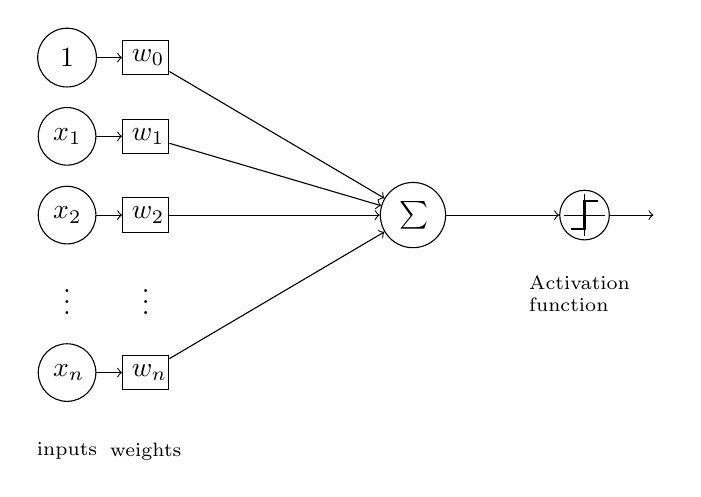
\begin{tikzpicture}
	
	\node[functions] (center) {};
        \node[below of=center,font=\scriptsize,text width=4em] {Activation function};
        \draw[thick] (0.5em,0.5em) -- (0,0.5em) -- (0,-0.5em) -- (-0.5em,-0.5em);
        \draw (0em,0.75em) -- (0em,-0.75em);
        \draw (0.75em,0em) -- (-0.75em,0em);
        \node[right of=center] (right) {};
            \path[draw,->] (center) -- (right);
        \node[functions,left=5em] (left) {$\sum$};
            \path[draw,->] (left) -- (center);
        \node[weights,left=15em] (2) {$w_2$} -- (2) node[input,left of=2] (l2) {$x_2$};
            \path[draw,->] (l2) -- (2);
            \path[draw,->] (2) -- (left);
        \node[below of=2] (dots) {$\vdots$} -- (dots) node[left of=dots] (ldots) {$\vdots$};
        \node[weights,below of=dots] (n) {$w_n$} -- (n) node[input,left of=n] (ln) {$x_n$};
            \path[draw,->] (ln) -- (n);
            \path[draw,->] (n) -- (left);
        \node[weights,above of=2] (1) {$w_1$} -- (1) node[input,left of=1] (l1) {$x_1$};
            \path[draw,->] (l1) -- (1);
            \path[draw,->] (1) -- (left);
        \node[weights,above of=1] (0) {$w_0$} -- (0) node[input,left of=0] (l0) {$1$};
            \path[draw,->] (l0) -- (0);
            \path[draw,->] (0) -- (left);
        \node[below of=ln,font=\scriptsize] {inputs};
        \node[below of=n,font=\scriptsize] {weights};
	
	\end{tikzpicture}
\caption{The perceptron model}
\label{perceptron_model}
\end{figure}

\subsection{Activation functions}
\label{activation_functions}
Once the computation of the weighted sum of all inputs for a specific neuron is done, the latter has to be pass the sum through an activation function that will decide the proportion of the result to send further. Activation functions have to be non-linear in order to approximate extremely complex functions. In fact, neural networks are considered as universal approximators. Article \cite{17} claims that "multilayer feedforward networks are capable of approximating any measurable function to any desired degree of accuracy, in a very specific and satisfying sense."According to \cite{18} the most commonly used activation functions are:\\\\
 \noindent \textbf{Sigmoid function}\\
 The sigmoid function is defined as:
 \begin{equation}
  g(x) = \frac{1}{1+e^{-x}}
 \end{equation}
 Its derivative is:
 \begin{equation}
 g'(x) = g(x)(1-g(x))
 \end{equation}
 


\begin{figure}[h!]
  \begin{center}
    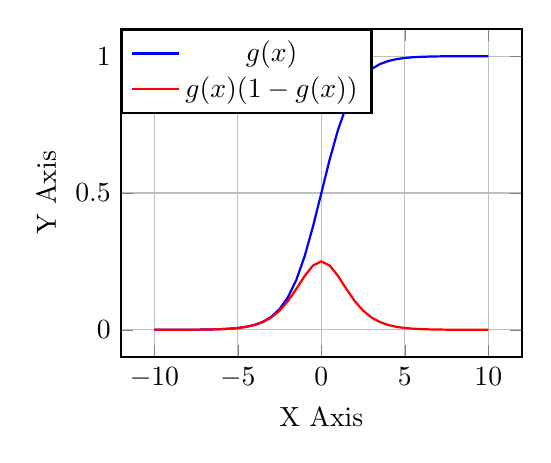
\begin{tikzpicture}
      \begin{axis}[
      	  width=0.55\linewidth, % Scale the plot to 0.7 \linewidth
          xlabel={$x$}, 
          ylabel={$y$},
          xlabel=X Axis, 
          ylabel=Y Axis,
          samples=41, 
          grid, 
          thick,
          domain=-10:10,
		legend style={at={(0,1)},anchor=north west}
        ]
        \addplot+[no marks] {1/(1+exp(-x))};
        \addlegendentry{$g(x)$}
        \addplot+[no marks] {(1/(1+exp(-x))) * (1-(1/(1+exp(-x))))};
        \addlegendentry{$g(x)(1-g(x))$}
      \end{axis}
    \end{tikzpicture}
    \caption{The sigmoid function and its derivative}
  \end{center}
\end{figure} 
 
 
 \noindent \textbf{Tanh function}\\
 \begin{equation}
 g(x) = tanh(x) = \frac{1-e^{-2x}}{1+e^{-2x}}
 \end{equation}
  
 Its derivative is:
 \begin{equation}
 g'(x) = tanh'(x) = 1-tanh^{2}(x)
 \end{equation}
 
  \begin{figure}[h!]
  \begin{center}
    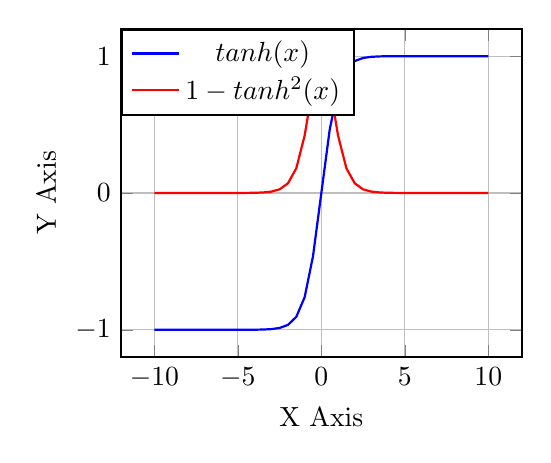
\begin{tikzpicture}
      \begin{axis}[
      	  width=0.55\linewidth, % Scale the plot to 0.7 \linewidth
          xlabel={$x$}, 
          ylabel={$y$},
          xlabel=X Axis, 
          ylabel=Y Axis,
          samples=41, 
          grid, 
          thick,
          domain=-10:10,
		legend style={at={(0,1)},anchor=north west}
        ]
        \addplot+[no marks] {(1-exp(-2*x))/(1+exp(-2*x))};
        \addlegendentry{$tanh(x)$}
        \addplot+[no marks] {1-((1-exp(-2*x))/(1+exp(-2*x)))^2};
        \addlegendentry{$1-tanh^{2}(x)$}
      \end{axis}
    \end{tikzpicture}
    \caption{The tanh function and its derivative}
  \end{center}
\end{figure} 
 
 \noindent \textbf{ReLU function}\\
 \begin{equation}
 g(x) = ReLU(x) = 
 \begin{cases}
    1 & \text{if } x\geq 0\\
    0              & \text{otherwise}
\end{cases}
 \end{equation}
 
 \begin{figure}[h!]
  \begin{center}
    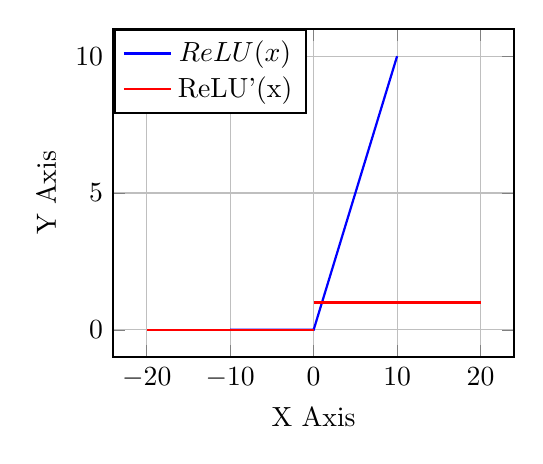
\begin{tikzpicture}[
    declare function={
    func(\x)= (\x<=0) * (0);
  }
  ]
      \begin{axis}[
      	  width=0.55\linewidth, % Scale the plot to 0.7 \linewidth
          xlabel={$x$}, 
          ylabel={$y$},
          xlabel=X Axis, 
          ylabel=Y Axis,
          samples=41, 
          grid, 
          thick,
          domain=-10:10,
		legend style={at={(0,1)},anchor=north west}
        ]
        \addplot+[no marks] {(x>=0)*x};
        \addlegendentry{$ReLU(x)$}
        \addplot[domain=-20:0,red] {0};
		\addplot[domain=0:20, red] {1};
        \addlegendentry{ReLU'(x)}
      \end{axis}
    \end{tikzpicture}
    \caption{The ReLU function and its derivative(not defined when x=0)}
  \end{center}
\end{figure} 
 
 
 
 
 \noindent \textbf{ELU function}\\
 \begin{equation}
 g(x) = 
 \begin{cases}
    x & \text{if } x\geq 0\\
    e^{x}-1 & \text{otherwise }
\end{cases}
 \end{equation}
  
 Its derivative is:
 \begin{equation}
g'(x) = 
 \begin{cases}
    1 & \text{if } x\geq 0\\
    e^{x} & \text{otherwise }
\end{cases}
 \end{equation}
 
 

  \begin{figure}[h!]
  \begin{center}
    \begin{tikzpicture}[
      \begin{axis}[
      	  width=0.55\linewidth, % Scale the plot to 0.7 \linewidth
          xlabel={$x$}, 
          ylabel={$y$},
          xlabel=X Axis, 
          ylabel=Y Axis,
          samples=41, 
          grid, 
          thick,
          domain=-10:10,
		legend style={at={(0,1)},anchor=north west}
        ]
        \addplot+[no marks] {func(x)};
        \addlegendentry{$ELU(x)$}
        \addplot+[no marks] {6};
        \addlegendentry{$ELU'(x)$}
      \end{axis}
    \end{tikzpicture}
    \caption{The ELU function and its derivative}
  \end{center}
\end{figure} 

\subsection{Multilayer perceptrons}
\label{multilayer_perceptron}
The figure \ref{multilayer_perceptrons_figure} globally illustrates the concept of a multilayer perceptrons: all inputs are given to all neurons of the first layer. Each neuron sums the incoming inputs, passes the result through a non linear function and sends it to all neuron of the next layer along an edge. Each edge between two neurons (i.e perceptrons) has a certain weight (a numerical value) that weights the importance of the output of the previous neuron.\\

\begin{figure}[!h]
\centering
	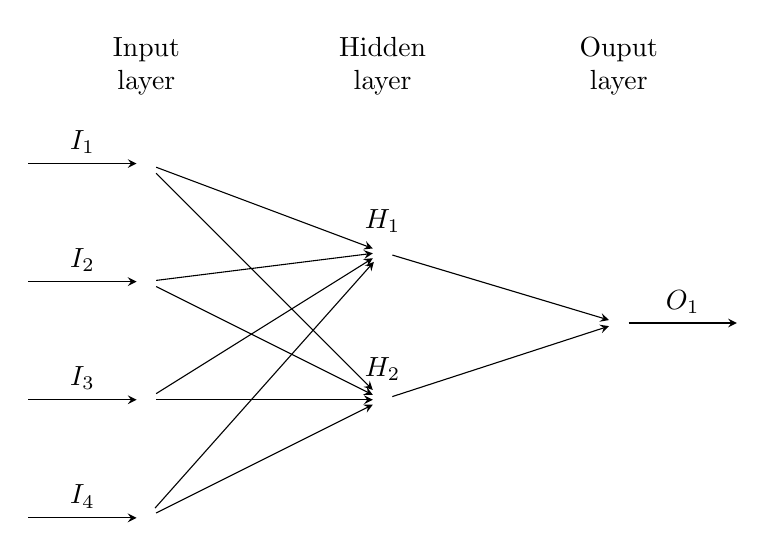
\begin{tikzpicture}[x=1.5cm, y=1.5cm, >=stealth]
	
	\foreach \m/\l [count=\y] in {1,2,3,4}
	  \node [every neuron/.try, neuron \m/.try] (input-\m) at (0,2.5-\y) {};
	
	\foreach \m [count=\y] in {1,2}
	  \node [every neuron/.try, neuron \m/.try ] (hidden-\m) at (2,2-\y*1.25) {};
	
	\foreach \m [count=\y] in {1}
	  \node [every neuron/.try, neuron \m/.try ] (output-\m) at (4,0.15) {};
	
	% input layer
	\foreach \l [count=\i] in {1,2,3,4}
	  \draw [<-] (input-\i) -- ++(-1,0)
	    node [above, midway] {$I_\l$};
	
	% hidden layer
	\foreach \l [count=\i] in {1,2}
	  \node [above] at (hidden-\i.north) {$H_\l$};
	
	% output neurons
	\foreach \l [count=\i] in {1}
	  \draw [->] (output-\i) -- ++(1,0)
	    node [above, midway] {$O_\l$};
	
	% input -> hidden
	\foreach \i in {1,...,4}
	  \foreach \j in {1,...,2}
	    \draw [->] (input-\i) -- (hidden-\j);
	
	% hidden -> output
	\foreach \i in {1,...,2}
	  \foreach \j in {1}
	    \draw [->] (hidden-\i) -- (output-\j);
	
	% labels above layers
	\foreach \l [count=\x from 0] in {Input, Hidden, Ouput}
	  \node [align=center, above] at (\x*2,2) {\l \\ layer};
	
	\end{tikzpicture}
\caption{Neural Network example}
\label{multilayer_perceptrons_figure}
\end{figure}


A multilayer perceptron is an artifical neural network type. Article \cite{22} defines the multilayer perceptrons in the following way: "Multilayer perceptron are feedforward networks with one or more layers of units between the
input and output layers. The output units represent a hyperplane in the space
of the input patterns."\\
A multilayer perceptrons is composed of multiple perceptrons that are arranged into multiple layers. When the input layer receives the signal, transmits it to the hidden layer



\subsection{Forward propagation}

\begin{figure}[!h]
\centering
\includegraphics[width=1\textwidth, keepaspectratio=true]{./figures/forward_propagation.png}
\caption{Forward propagation }
\label{forward_propagation}
\end{figure}


\subsection{Backpropagation}

\subsubsection{Loss function}

\subsubsection{Weight update}




\section{Training a neural network}

\subsection{Data}
Training set, validation set, test set, supervised learning, unsupervised learning,

\subsection{Weight initialization}

\subsection{Hyperparameters}
lr, batch size, epochs, optimizer, learning rate decay, ...




\section{Deep learning models}
xxx

\subsubsection{Convolutional Neural Networks}


\subsubsection{Recurrent Neural Networks}




\section{Transfer learning}




\section{Deep learning frameworks}